\documentclass{ximera}
\usepackage{epsfig}

\graphicspath{
  {./}
  {figures/}
}

\usepackage{epstopdf}
%\usepackage{ulem}
\usepackage[normalem]{ulem}

\epstopdfsetup{outdir=./}

\usepackage{morewrites}
\makeatletter
\newcommand\subfile[1]{%
\renewcommand{\input}[1]{}%
\begingroup\skip@preamble\otherinput{#1}\endgroup\par\vspace{\topsep}
\let\input\otherinput}
\makeatother

\newcommand{\EXER}{}
\newcommand{\includeexercises}{\EXER\directlua{dofile(kpse.find_file("exercises","lua"))}}

\newenvironment{computerExercise}{\begin{exercise}}{\end{exercise}}

%\newcounter{ccounter}
%\setcounter{ccounter}{1}
%\newcommand{\Chapter}[1]{\setcounter{chapter}{\arabic{ccounter}}\chapter{#1}\addtocounter{ccounter}{1}}

%\newcommand{\section}[1]{\section{#1}\setcounter{thm}{0}\setcounter{equation}{0}}

%\renewcommand{\theequation}{\arabic{chapter}.\arabic{section}.\arabic{equation}}
%\renewcommand{\thefigure}{\arabic{chapter}.\arabic{figure}}
%\renewcommand{\thetable}{\arabic{chapter}.\arabic{table}}

%\newcommand{\Sec}[2]{\section{#1}\markright{\arabic{ccounter}.\arabic{section}.#2}\setcounter{equation}{0}\setcounter{thm}{0}\setcounter{figure}{0}}
  
\newcommand{\Sec}[2]{\section{#1}}

\setcounter{secnumdepth}{2}
%\setcounter{secnumdepth}{1} 

%\newcounter{THM}
%\renewcommand{\theTHM}{\arabic{chapter}.\arabic{section}}

\newcommand{\trademark}{{R\!\!\!\!\!\bigcirc}}
%\newtheorem{exercise}{}

\newcommand{\dfield}{{\sf SlopeField}}

\newcommand{\pplane}{{\sf PhasePlane}}

\newcommand{\PPLANE}{{\sf PHASEPLANE}}

% BADBAD: \newcommand{\Bbb}{\bf}. % Package amsfonts Warning: Obsolete command \Bbb; \mathbb should be used instead.

\newcommand{\R}{\mbox{$\mathbb{R}$}}
\let\C\relax
\newcommand{\C}{\mbox{$\mathbb{C}$}}
\newcommand{\Z}{\mbox{$\mathbb{Z}$}}
\newcommand{\N}{\mbox{$\mathbb{N}$}}
\newcommand{\D}{\mbox{{\bf D}}}

\newcommand{\WW}{\mathcal{W}}

\usepackage{amssymb}
%\newcommand{\qed}{\hfill\mbox{\raggedright$\square$} \vspace{1ex}}
%\newcommand{\proof}{\noindent {\bf Proof:} \hspace{0.1in}}

\newcommand{\setmin}{\;\mbox{--}\;}
\newcommand{\Matlab}{{M\small{AT\-LAB}} }
\newcommand{\Matlabp}{{M\small{AT\-LAB}}}
\newcommand{\computer}{\Matlab Instructions}
\renewcommand{\computer}{M\small{ATLAB} Instructions}
\newcommand{\half}{\mbox{$\frac{1}{2}$}}
\newcommand{\compose}{\raisebox{.15ex}{\mbox{{\scriptsize$\circ$}}}}
\newcommand{\AND}{\quad\mbox{and}\quad}
\newcommand{\vect}[2]{\left(\begin{array}{c} #1_1 \\ \vdots \\
 #1_{#2}\end{array}\right)}
\newcommand{\mattwo}[4]{\left(\begin{array}{rr} #1 & #2\\ #3
&#4\end{array}\right)}
\newcommand{\mattwoc}[4]{\left(\begin{array}{cc} #1 & #2\\ #3
&#4\end{array}\right)}
\newcommand{\vectwo}[2]{\left(\begin{array}{r} #1 \\ #2\end{array}\right)}
\newcommand{\vectwoc}[2]{\left(\begin{array}{c} #1 \\ #2\end{array}\right)}

\newcommand{\ignore}[1]{}


\newcommand{\inv}{^{-1}}
\newcommand{\CC}{{\cal C}}
\newcommand{\CCone}{\CC^1}
\newcommand{\Span}{{\rm span}}
\newcommand{\rank}{{\rm rank}}
\newcommand{\trace}{{\rm tr}}
\newcommand{\RE}{{\rm Re}}
\newcommand{\IM}{{\rm Im}}
\newcommand{\nulls}{{\rm null\;space}}

\newcommand{\dps}{\displaystyle}
\newcommand{\arraystart}{\renewcommand{\arraystretch}{1.8}}
\newcommand{\arrayfinish}{\renewcommand{\arraystretch}{1.2}}
\newcommand{\Start}[1]{\vspace{0.08in}\noindent {\bf Section~\ref{#1}}}
\newcommand{\exer}[1]{\noindent {\bf \ref{#1}}}
\newcommand{\ans}{\textbf{Answer:} }
\newcommand{\matthree}[9]{\left(\begin{array}{rrr} #1 & #2 & #3 \\ #4 & #5 & #6
\\ #7 & #8 & #9\end{array}\right)}
\newcommand{\cvectwo}[2]{\left(\begin{array}{c} #1 \\ #2\end{array}\right)}
\newcommand{\cmatthree}[9]{\left(\begin{array}{ccc} #1 & #2 & #3 \\ #4 & #5 &
#6 \\ #7 & #8 & #9\end{array}\right)}
\newcommand{\vecthree}[3]{\left(\begin{array}{r} #1 \\ #2 \\
#3\end{array}\right)}
\newcommand{\cvecthree}[3]{\left(\begin{array}{c} #1 \\ #2 \\
#3\end{array}\right)}
\newcommand{\cmattwo}[4]{\left(\begin{array}{cc} #1 & #2\\ #3
&#4\end{array}\right)}

\newcommand{\Matrix}[1]{\ensuremath{\left(\begin{array}{rrrrrrrrrrrrrrrrrr} #1 \end{array}\right)}}

\newcommand{\Matrixc}[1]{\ensuremath{\left(\begin{array}{cccccccccccc} #1 \end{array}\right)}}



\renewcommand{\labelenumi}{\theenumi}
\newenvironment{enumeratea}%
{\begingroup
 \renewcommand{\theenumi}{\alph{enumi}}
 \renewcommand{\labelenumi}{(\theenumi)}
 \begin{enumerate}}
 {\end{enumerate}
 \endgroup}

\newcounter{help}
\renewcommand{\thehelp}{\thesection.\arabic{equation}}

%\newenvironment{equation*}%
%{\renewcommand\endequation{\eqno (\theequation)* $$}%
%   \begin{equation}}%
%   {\end{equation}\renewcommand\endequation{\eqno \@eqnnum
%$$\global\@ignoretrue}}

%\input{psfig.tex}

\author{Martin Golubitsky and Michael Dellnitz}

%\newenvironment{matlabEquation}%
%{\renewcommand\endequation{\eqno (\theequation*) $$}%
%   \begin{equation}}%
%   {\end{equation}\renewcommand\endequation{\eqno \@eqnnum
% $$\global\@ignoretrue}}

\newcommand{\soln}{\textbf{Solution:} }
\newcommand{\exercap}[1]{\centerline{Figure~\ref{#1}}}
\newcommand{\exercaptwo}[1]{\centerline{Figure~\ref{#1}a\hspace{2.1in}
Figure~\ref{#1}b}}
\newcommand{\exercapthree}[1]{\centerline{Figure~\ref{#1}a\hspace{1.2in}
Figure~\ref{#1}b\hspace{1.2in}Figure~\ref{#1}c}}
\newcommand{\para}{\hspace{0.4in}}

\usepackage{ifluatex}
\ifluatex
\ifcsname displaysolutions\endcsname%
\else
\renewenvironment{solution}{\suppress}{\endsuppress}
\fi
\else
\renewenvironment{solution}{}{}
\fi

\ifcsname answer\endcsname
\renewcommand{\answer}{}
\fi

%\ifxake
%\newenvironment{matlabEquation}{\begin{equation}}{\end{equation}}
%\else
\newenvironment{matlabEquation}%
{\let\oldtheequation\theequation\renewcommand{\theequation}{\oldtheequation*}\begin{equation}}%
  {\end{equation}\let\theequation\oldtheequation}
%\fi

\makeatother

\newcommand{\RED}[1]{{\color{red}{#1}}} 

\begin{document}

\noindent In Exercises~\ref{c8.4.5a} -- \ref{c8.4.5b} answer the following 
four questions for the given system of differential equations:
\begin{itemize}
\item[(a)]  How many equilibria does the system of differential equations 
have?  Any equilibrium that you find using {\pplane} may be considered an 
actual equilibrium.  But use analysis to prove that you have found them all.
\item[(b)]  How many limit cycles does the system of differential equations 
have?  Base your answer on numerical exploration using {\pplane}.
\item[(c)]  By hand (and not necessarily to scale) sketch the phase portrait.
\item[(d)]  Indicate which initial conditions have solutions that stay
bounded in forward time.
\end{itemize}
\begin{computerExercise}  \label{c8.4.5a}
\begin{matlabEquation}\label{MATLAB:4}
\begin{array}{rcl}
\dot{x} & = & 0.04x - y - 3y^2 + 2.5xy\\
\dot{y} & = & x - 3x^2 + 2x^2y.
\end{array}
\end{matlabEquation}

\begin{solution}

\ans There are five equilibria and two limit cycles.  The phase portrait is
given in Figure~\ref{c8.4.5a}a.  The orbits that stay bounded in
forward time are indicated in Figure~\ref{c8.4.5a}b.

\soln (a)  Using {\pplane} we can find five equilibria
\begin{verbatim}
(0.0000, 0.0000)        Spiral source.           
(1.8519, 1.2300)        Nodal source.            
(0.3445, 0.0485)        Saddle point.            
(0.3102, -0.1118)       Spiral sink.             
(0.0000, -0.3333)       Saddle point.            
\end{verbatim}
We can show that there are at most five equilibria by solving:
\begin{eqnarray*}
0.04x - y - 3y^2 + 2.5xy & = & 0\\
x - 3x^2 + 2x^2y & = & 0.
\end{eqnarray*}  
Factoring the second equation leads to 
\[
x=0 \quad \mbox{ or } \quad x = \frac{1}{3-2y}.
\]
Substituting $x=0$ into the first equation leads to the equilibria
$(0,0)$ and $(0,-\frac{1}{3})$. Substituting $x = \frac{1}{3-2y}$ into the
first equation yields
\[
\frac{0.04+2.5y}{3-2y} -(y+3y^2)=0.
\]
Multiplying this equation by $3-2y$ leads to a cubic equation that has at most
three roots.  Thus there are at most five equilibria in this system of
differential equations.

\noindent (b) There is numerical evidence for two limit cycles
one surrounding the spiral source at the origin and one surrounding the
spiral sink at $(0.3102, -0.1118)$.

\noindent (c)  The five equilibria, two limit cycles, and the stable and
unstable orbits of saddles are shown in Figure~\ref{c8.4.5a}a.

\noindent (d)  The solutions that stay bounded in forward time include the
equilibria, limit cycle and those indicated in Figure~\ref{c8.4.5a}b.

\begin{figure}[htb]
                       \centerline{%
                        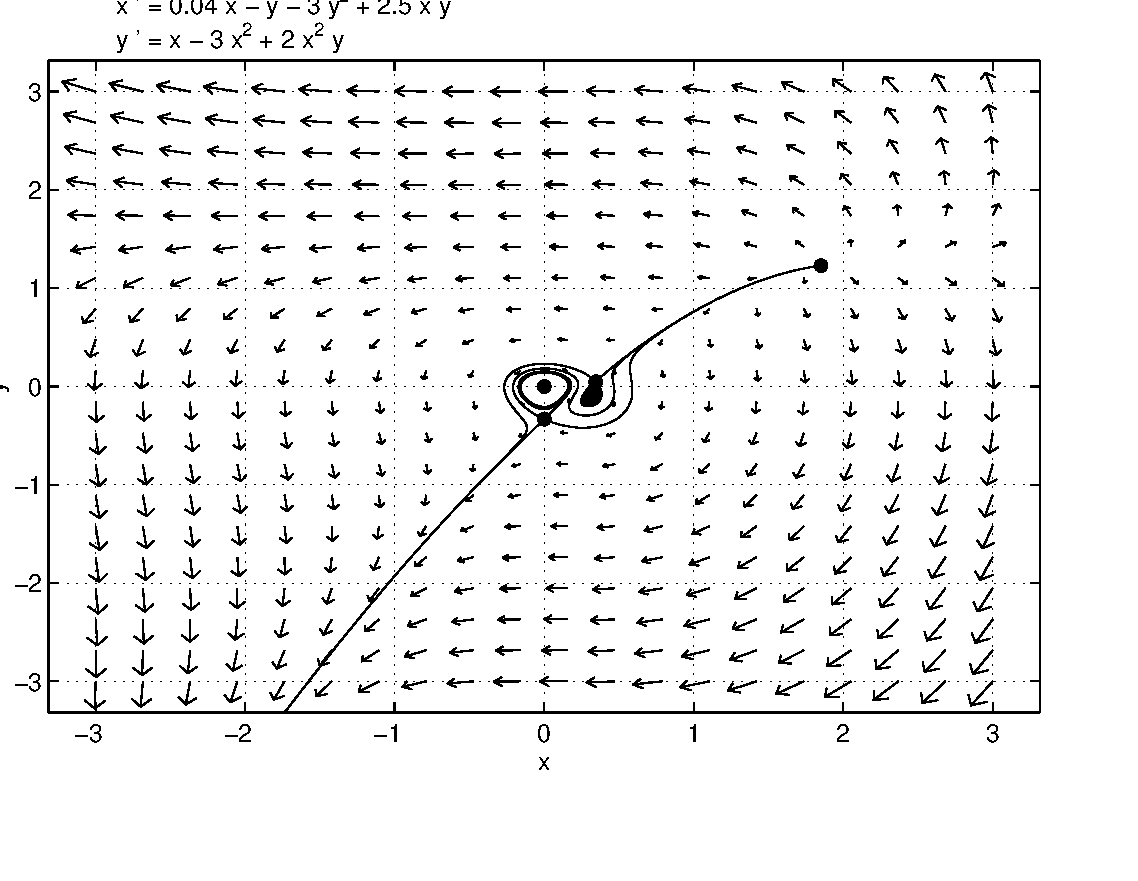
\includegraphics[width=2.75in]{exfigure/8-4-5a.pdf}
			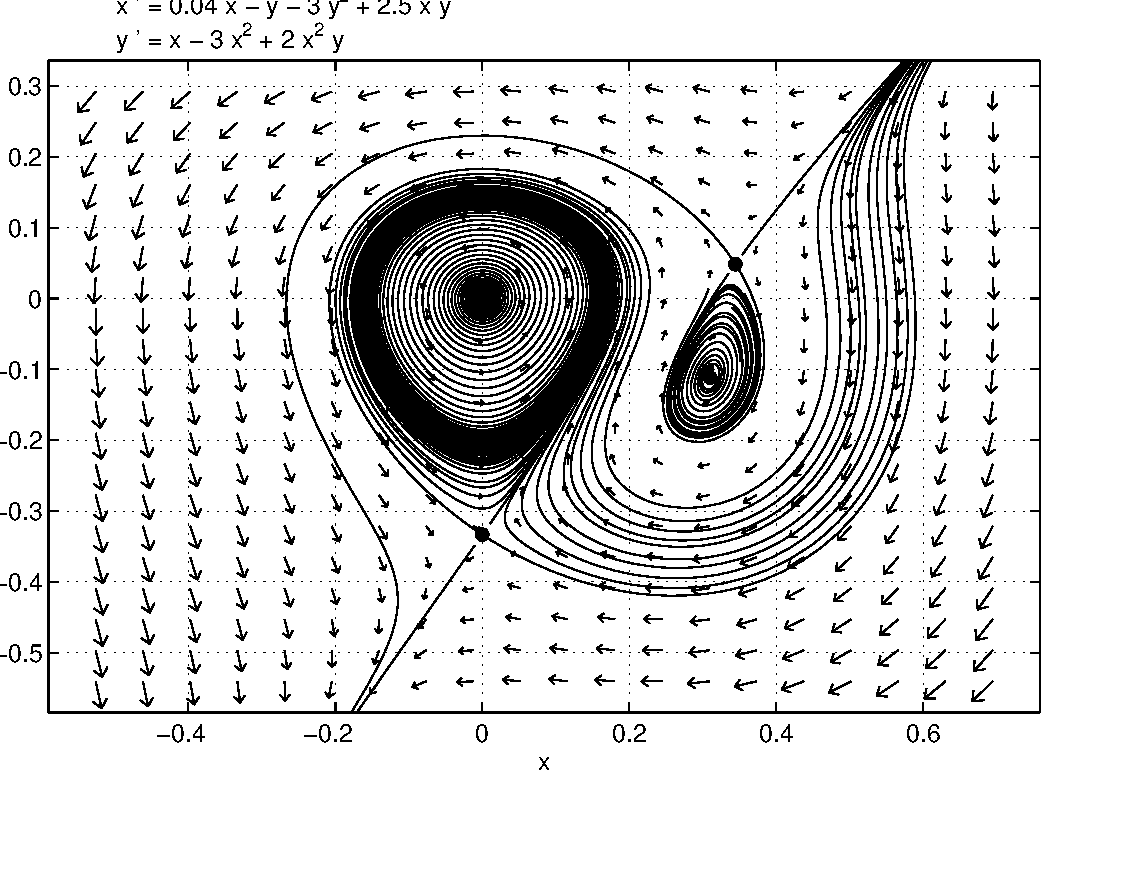
\includegraphics[width=2.75in]{exfigure/8-4-5a2.pdf}}
                \exercaptwo{c8.4.5a}
\end{figure}




\end{solution}
\end{computerExercise}
\begin{computerExercise}  \label{c8.4.5b}
\begin{matlabEquation}\label{MATLAB:5}
\begin{array}{rcl}
\dot{x} & = & 0.05x - y - 3y^2 + 2xy \\
\dot{y} & = & x - 3x^2 + x^2y.
\end{array}
\end{matlabEquation}

\begin{solution}

\ans There are five equilibria and one limit cycle.  The phase portrait is
given in Figure~\ref{c8.4.5b}a.  The orbits that stay bounded in forward time
are indicated in Figure~\ref{c8.4.5b}b.

\soln  (a)  Using {\pplane} we can find five equilibria
\begin{verbatim}
(0.0000, 0.0000)        Spiral source.           
(4.6347, 2.7842)        Nodal source.            
(0.3377, 0.0384)        Saddle point.            
(0.3169, -0.1560)       Spiral sink.             
(0.0000, -0.3333)       Saddle point.            
\end{verbatim}
We can show that there are at most five equilibria by solving:
\begin{eqnarray*}
0.05x - y - 3y^2 + 2xy & = & 0\\
x - 3x^2 + x^2y & = & 0.
\end{eqnarray*}  
Factoring the second equation leads to 
\[
x=0 \quad \mbox{ or } \quad x = \frac{1}{3-y}.
\]
Substituting $x=0$ into the first equation leads to the equilibria
$(0,0)$ and $(0,-\frac{1}{3})$. Substituting $x = \frac{1}{3-y}$ into the
first equation yields
\[
\frac{0.05+2y}{3-y} -(y+3y^2)=0.
\]
Multiplying this equation by $3-y$ leads to a cubic equation that has at most
three roots.  Thus there are at most five equilibria in this system of
differential equations.

\noindent (b) There is numerical evidence for just one limit cycle
surrounding the equilibrium at the origin.

\noindent (c)  The five equilibria, one limit cycle, and the stable and
unstable orbits of saddles are shown in Figure~\ref{c8.4.5b}a.

\noindent (d)  The solutions that stay bounded in forward time include the
equilibria, limit cycle and those indicated in Figure~\ref{c8.4.5b}b.

\begin{figure}[htb]
                       \centerline{%
                        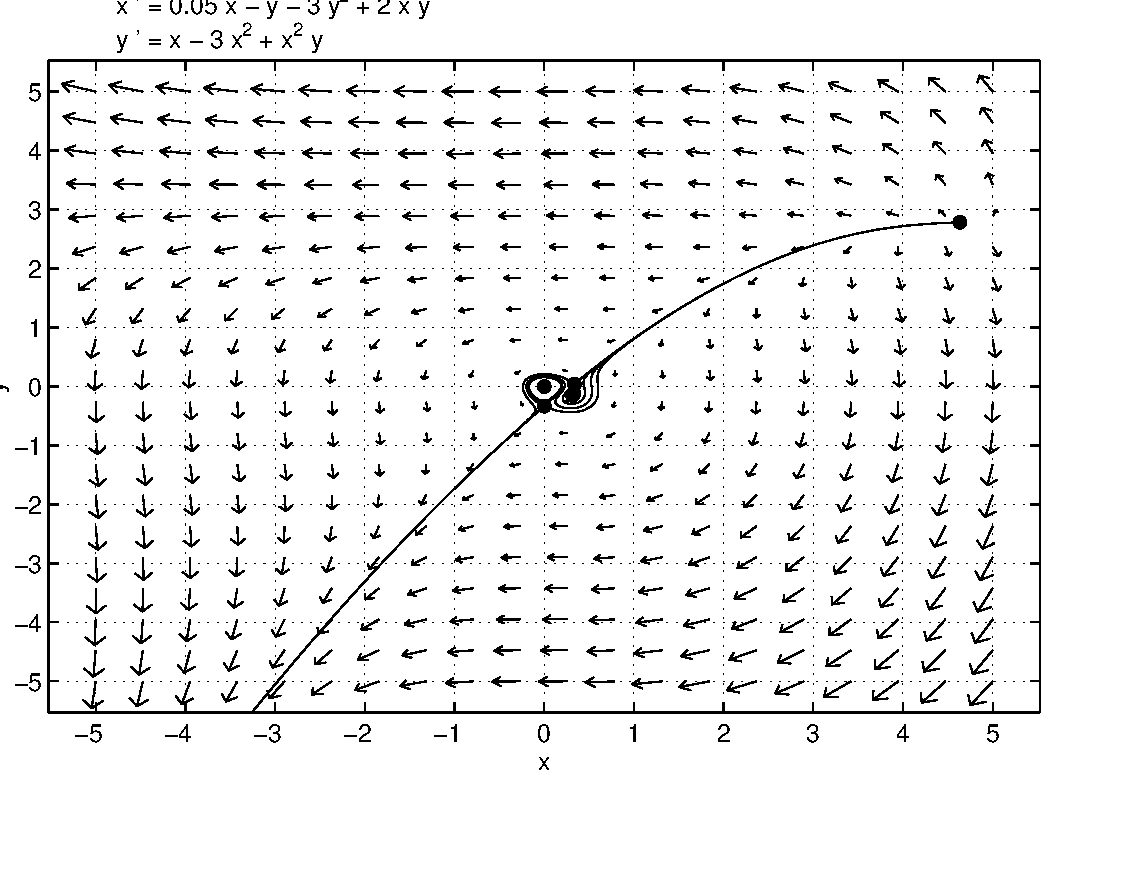
\includegraphics[width=2.75in]{exfigure/8-4-5b.pdf}
			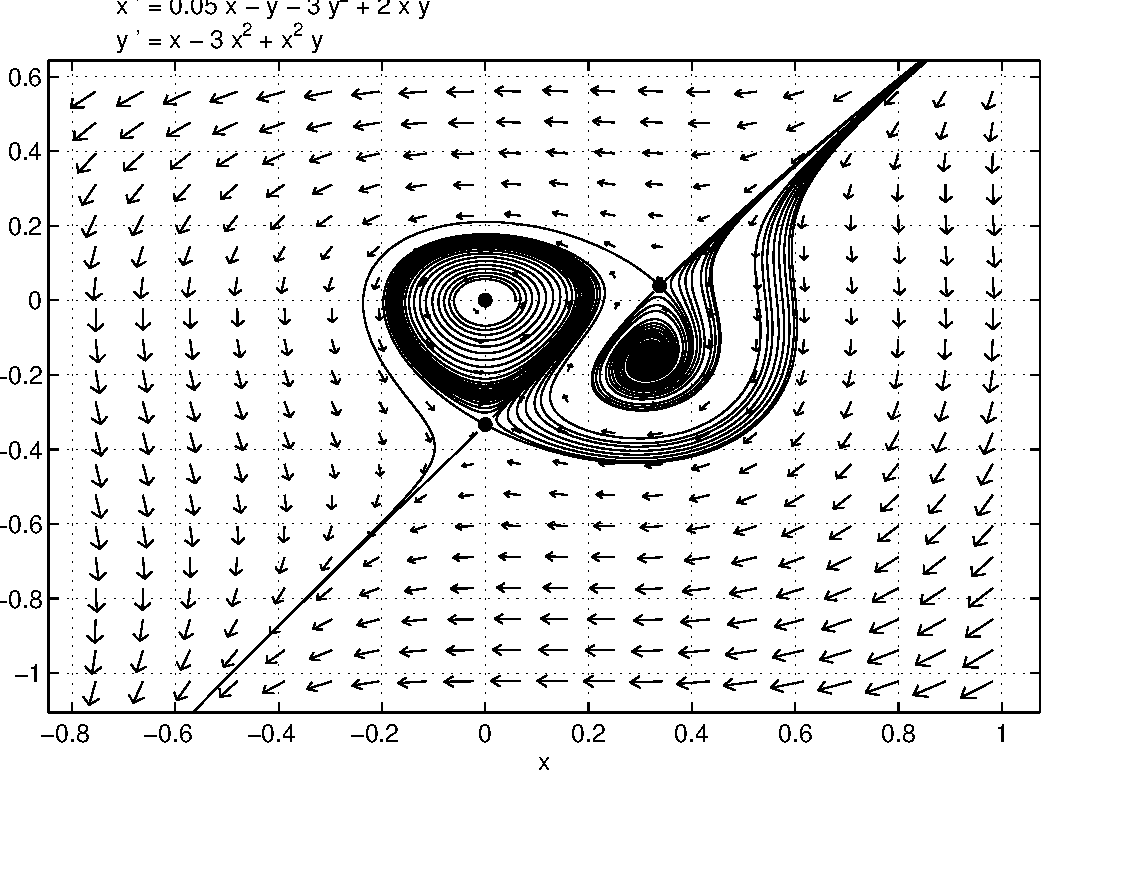
\includegraphics[width=2.75in]{exfigure/8-4-5b2.pdf}}
                \exercaptwo{c8.4.5b}
\end{figure}



\end{solution}
\end{computerExercise}
\end{document}
